\section{Môi trường thực nghiệm, bộ dữ liệu và các chỉ số đánh giá}
\label{sec:moi_truong_du_lieu_chi_so}

\subsection{Cấu hình môi trường thực nghiệm và liêm chính tái lập}

Toàn bộ thực nghiệm được thực thi trên cấu hình đồng nhất: vi xử lý đa nhân x86\_64 (AVX2), RAM $16.0\text{ GiB}$, hệ điều hành Windows 11 64-bit, Python \texttt{3.13.12} (\texttt{numpy 2.5.4}, \texttt{scipy 1.18.1}, \texttt{scikit-image 0.26.0}, \texttt{scikit-learn 1.9.1}, \texttt{matplotlib 3.11.2}, \texttt{Pillow 13.0.0}). Các thư viện đại số tuyến tính được khóa đơn luồng (\texttt{OMP/MKL/OPENBLAS\_NUM\_THREADS=1}), cố định hạt giống $\texttt{seed} = 2026$ và kiểm chứng toàn vẹn qua mã băm \texttt{manifest\_sha256} trong \texttt{results/sos/run\_manifest.json}.

\subsection{Bộ dữ liệu chuẩn Refined Deep-SAR Oil Spill (SOS)}

Nghiên cứu sử dụng bộ dữ liệu công khai \textit{Refined Deep-SAR Oil Spill (SOS)}~\cite{zuenko2025refined}, kế thừa từ công trình của Zhu và cộng sự~\cite{zhu2022oil}, gồm 21 cảnh SAR độ phân giải cao từ hai sự cố tràn dầu lớn được cắt thành các mảnh $256 \times 256$ điểm ảnh (Bảng~\ref{tab:thong_ke_sos}):
\begin{enumerate}
    \item \textbf{Mỏ dầu Al-Khafji (Vịnh Ba Tư, 2017):} 7 cảnh vệ tinh Sentinel-1A (băng C, $\sim 5.6\text{ cm}$, phân cực VV, chế độ IW mức GRD, độ phân giải $5\text{ m} \times 20\text{ m}$).
    \item \textbf{Giàn khoan Deepwater Horizon (Vịnh Mexico, 2010):} 14 cảnh vệ tinh ALOS PALSAR (băng L, $\sim 23.6\text{ cm}$, phân cực HH, mức 1.5, độ phân giải $12.5\text{ m}$).
\end{enumerate}

\begin{table}[!htbp]
\centering
\small
\caption{Thống kê phân chia các tập dữ liệu trong nghiên cứu.}
\label{tab:thong_ke_sos}
\resizebox{\textwidth}{!}{%
\begin{tabular}{|l|c|c|p{6.0cm}|}
\hline
\textbf{Phân tập dữ liệu} & \textbf{Cảm biến vệ tinh} & \textbf{Số lượng ảnh} & \textbf{Vai trò và mục đích sử dụng} \\ \hline
\textbf{Train (Huấn luyện)} & Sentinel-1A & $2\,683$ ảnh & Trích xuất mẫu huấn luyện LinearSVM và CART, tính thống kê Z-score. \\ \hline
\textbf{Validation (Kiểm định)} & Sentinel-1A & $671$ ảnh & Độc quyền phục vụ sàng lọc 110 cấu hình lọc/ngưỡng và 729 cấu hình mô hình vùng. \\ \hline
\textbf{Test (Kiểm thử độc lập)} & Sentinel-1A & $839$ ảnh & Đánh giá khách quan cấu hình chiến thắng sau khi toàn bộ quy trình đã đóng băng. \\ \hline
\textbf{External Test (Ngoài cảm biến)} & ALOS PALSAR & $776$ ảnh & Kiểm tra khả năng chuyển giao ngoài miền cảm biến với mô hình đóng băng từ Sentinel-1A. \\ \hline
\textbf{Tổng cộng sử dụng} & \multicolumn{3}{c|}{\textbf{4\,969 ảnh viễn thám $256 \times 256$}} \\ \hline
\end{tabular}%
}
\end{table}

\subsection{Giao thức phân tầng theo 5 chế độ diện tích dầu}

Dựa trên tỷ lệ diện tích dầu $r = \frac{1}{HW}\sum_{x,y} G(x, y)$ trên mặt nạ Ground Truth, các ảnh được phân tầng thành 5 chế độ ($R_0 \to R_4$): \textbf{$R_0$ (Biển sạch, $r = 0$)} kiểm định tỷ lệ báo nhầm; \textbf{$R_1$ (Vết dầu nhỏ, $0 < r < 0.05$)}; \textbf{$R_2$ (Dải dầu trung bình, $0.05 \le r < 0.50$)}; \textbf{$R_3$ (Dầu diện rộng, $0.50 \le r < 0.95$)}; và \textbf{$R_4$ (Ngập dầu toàn phần, $r \ge 0.95$)}. Hình~\ref{fig:sos_dataset_regimes} cho thấy histogram hai đỉnh phân tách rõ chỉ xuất hiện ở $R_2$, trong khi ở $R_0$ và $R_4$, histogram đơn đỉnh khiến ngưỡng Otsu thô bị ép chia đôi ảnh và sinh ra các đốm báo nhầm.

\begin{figure}[!htbp]
\centering
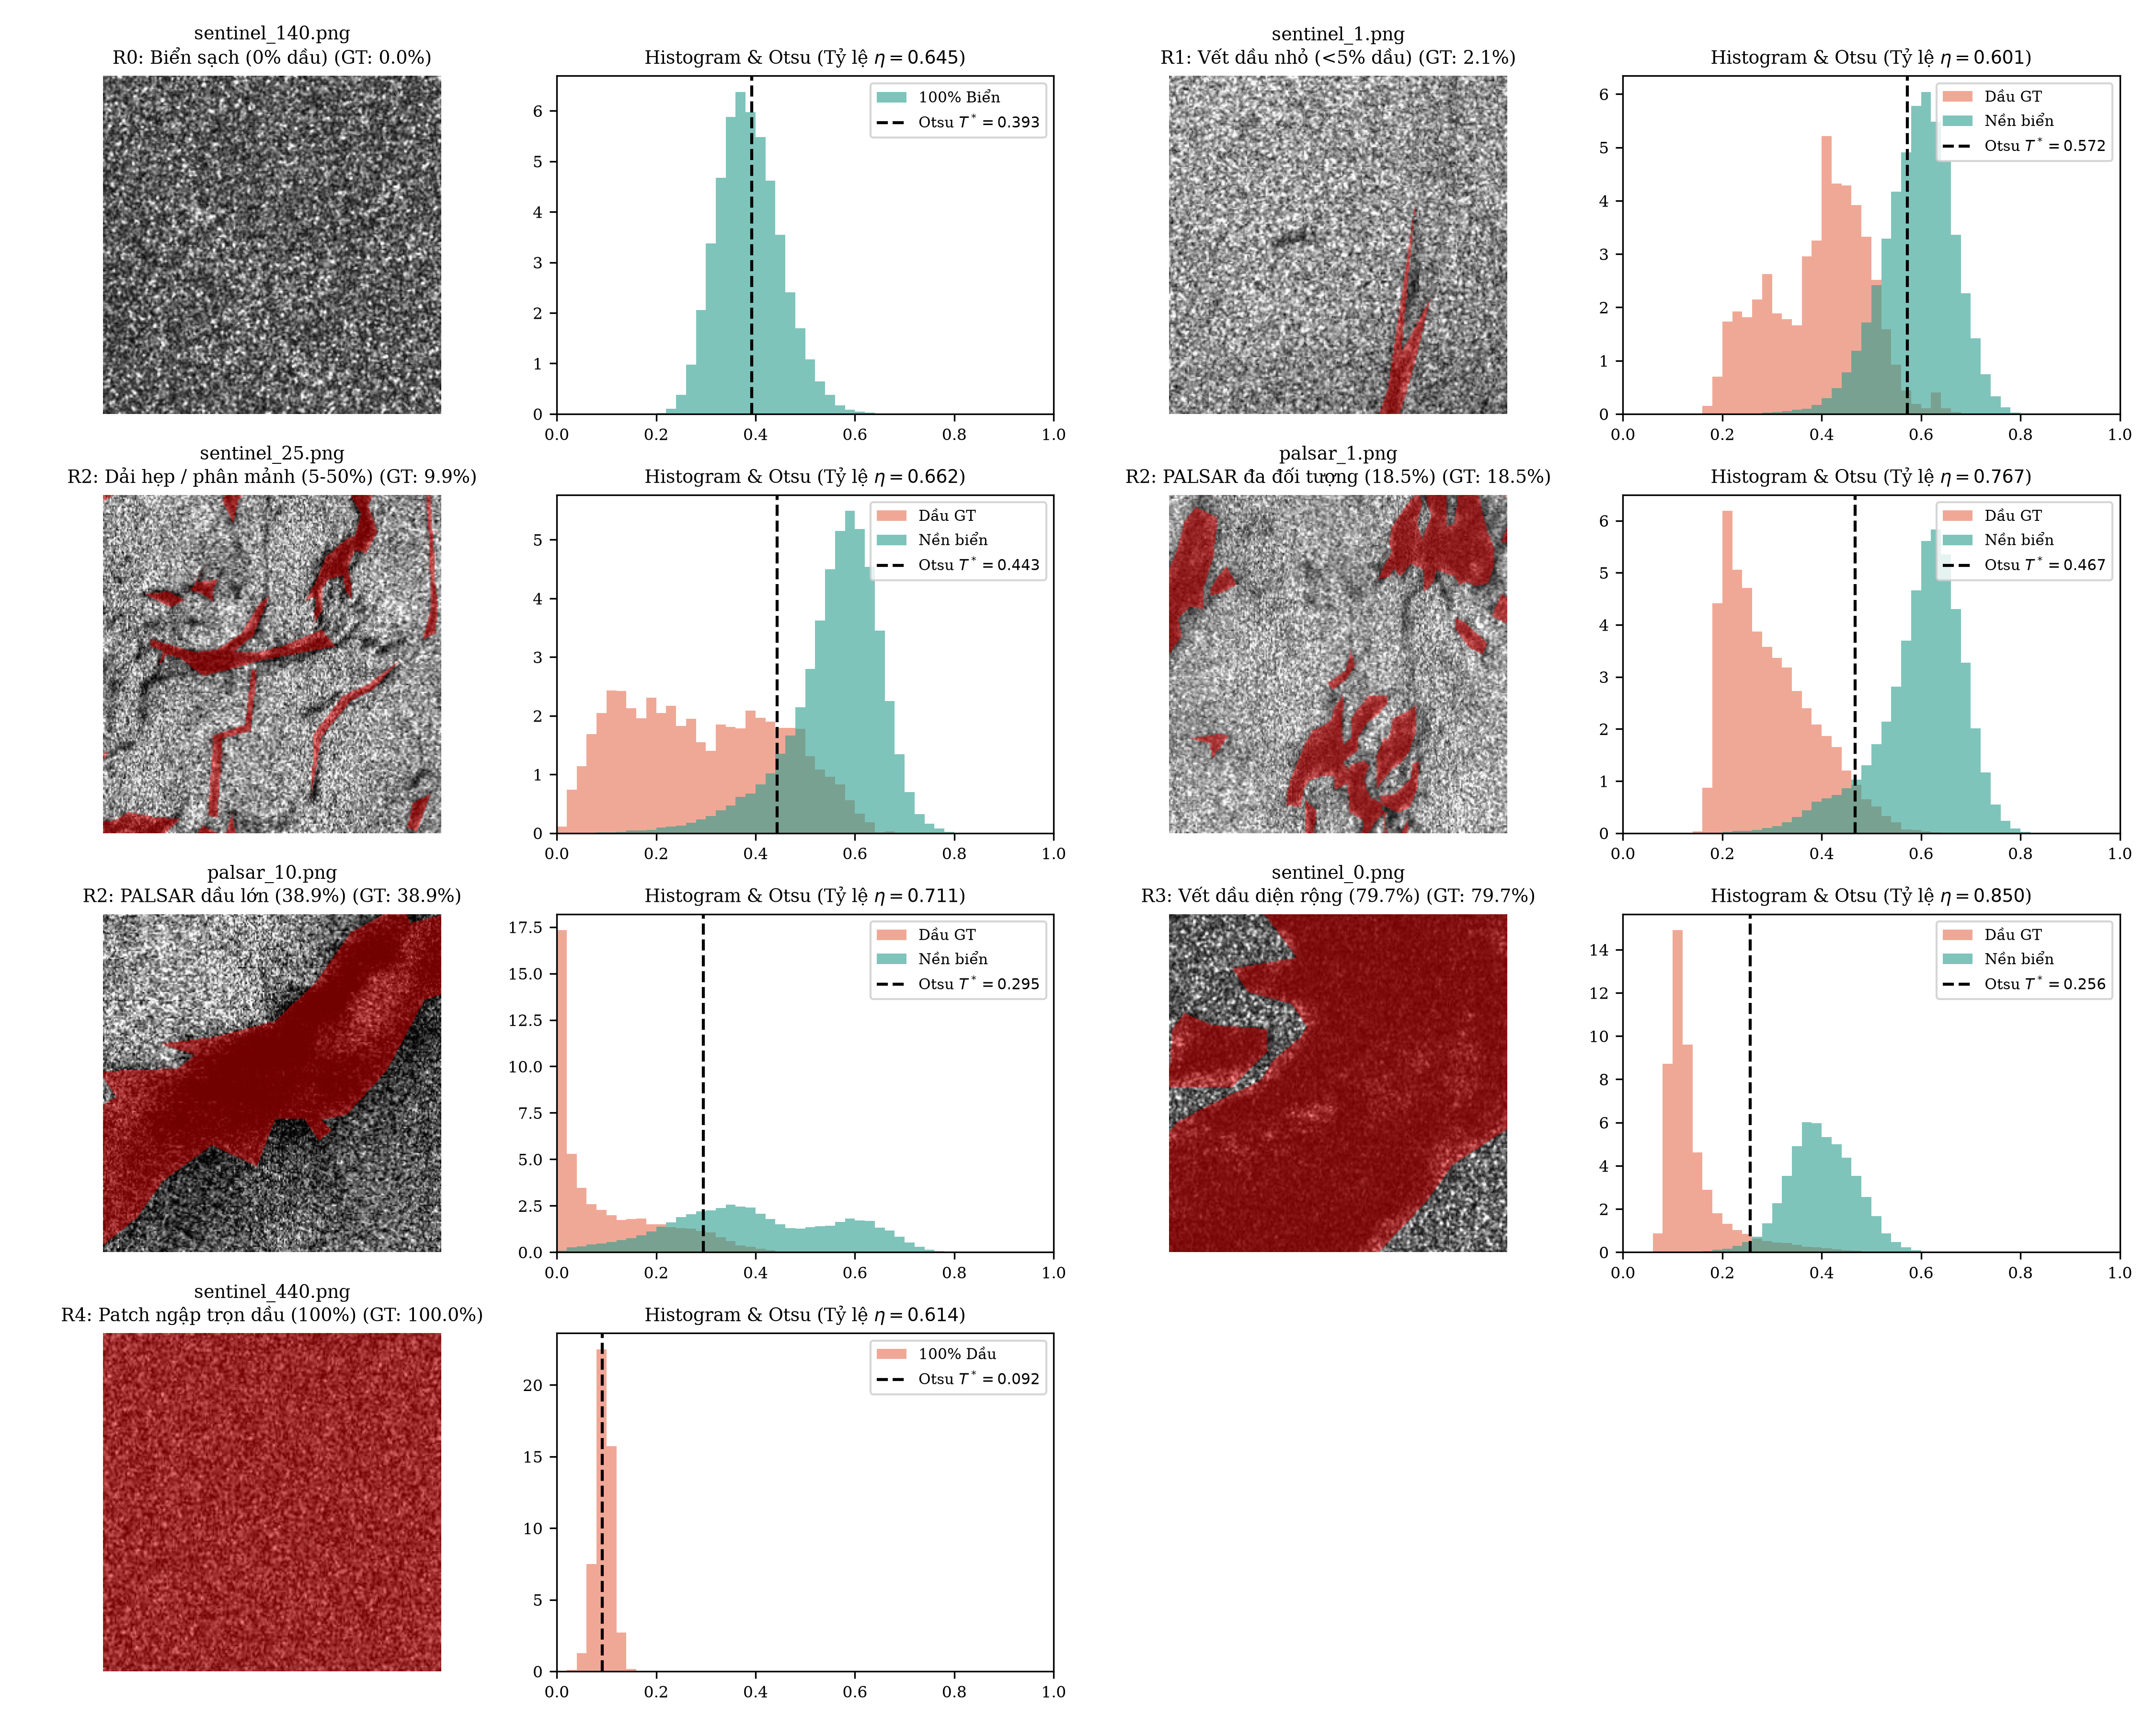
\includegraphics[width=0.90\textwidth]{figures/fig2_sos_dataset_regimes.png}
\caption{Mẫu ảnh SAR thực tế, mặt nạ Ground Truth và phân bố biểu đồ mức xám histogram qua 5 chế độ diện tích dầu ($R_0 \to R_4$).}
\label{fig:sos_dataset_regimes}
\end{figure}

\subsection{Hệ thống các chỉ số đánh giá định lượng}

Nghiên cứu áp dụng đồng thời hai cấp độ đánh giá độc lập:
\begin{enumerate}
    \item \textbf{Đánh giá cấp đối tượng theo thuật toán Hungarian ($\IoU \ge 0.5$):}
    Mặt nạ dự đoán $\hat{M}$ và Ground Truth $G$ được phân rã thành các đối tượng liên thông $\{\hat{\Omega}_p\}_{p=1}^P$ và $\{G_q\}_{q=1}^Q$. Ma trận $\IoU_{p, q} = |\hat{\Omega}_p \cap G_q| / |\hat{\Omega}_p \cup G_q|$ được giải ghép cặp một-một bằng thuật toán Hungarian; cặp đạt $\IoU_{p, q} \ge 0.5$ được tính là True Positive (TP), vùng dự đoán dư là False Positive (FP), và đối tượng bỏ sót là False Negative (FN). Các chỉ số vi mô (Micro-averaging) trên toàn tập ảnh gồm:
    \begin{equation}
    \text{Precision} = \frac{\sum \text{TP}}{\sum \text{TP} + \sum \text{FP}}, \quad \text{Recall} = \frac{\sum \text{TP}}{\sum \text{TP} + \sum \text{FN}}, \quad \text{Object F1} = \frac{2 \sum \text{TP}}{2 \sum \text{TP} + \sum \text{FP} + \sum \text{FN}}
    \end{equation}
    Ngoài ra, nghiên cứu báo cáo trung bình vĩ mô từng ảnh ($\text{mean} \pm \text{SD}$), tỷ lệ thu hồi vùng chạm biên (\textbf{Edge Recall}) và vùng nội bộ (\textbf{Interior Recall}).
    \item \textbf{Đánh giá cấp điểm ảnh (Pixel-level) và mật độ cảnh báo sai:}
    Độ bao phủ diện tích toàn cục và số vùng báo nhầm trung bình mỗi ảnh (\textbf{FP/ảnh}) được tính bởi:
    \begin{equation}
    \text{Pixel IoU} = \frac{\sum |\hat{M} \cap G|}{\sum |\hat{M} \cup G|}, \quad \text{Dice} = \frac{2 \sum |\hat{M} \cap G|}{\sum |\hat{M}| + \sum |G|}
    \end{equation}
\end{enumerate}
